$\quad\;\:$В данном разделе описаны эксперименты с регуляризацией тематических моделей в BigARTM. Ставится задача повторить как можно более похоже эксперименты, проведённые в \cite{voron_potap_14}.

\subsection{Описание экспериментов}

Использовалась коллекция NIPS в виде <<мешка слов>>, объём словаря $\approx$ 13000 терминов без предобработки. Количество документов --- около 1500. Эксперименты имеют общие параметры:

\vspace{5pt}

\begin{enumerate}
 \item Число проходов по коллекции --- 40;
 \item Число проходов по блоку --- 1;
 \item Число блоков --- 3;
 \item Число проходов по документу --- 1;
 \item Число документов --- 1500;
 \item Размер блока документов --- 500;
 \item Число предметных тем --- 90;
 \item Число фоновых тем --- 10;
 \item Порог нулевого значения --- 1е-100;
\end{enumerate}

{\bf Замечание: }В экспериментах, в которых фоновые и предметные темы не различались все темы считаются предметными. Если же темы различны, то степень разреженности оценивается по столбцам (строкам), соответствующим предметным темам. Аналогично, уникальности слов в топах рассматривались только в предметных темах. Декоррелятор тем так же работает только с предметными темами.

\vspace{5pt}

Критериями качества обучения являлись перплексия на обучающей выборке, разреженность матриц $\Phi$ и $\Theta$ и процент уникальных среди десяти и ста наиболее вероятных слов в каждой теме, объединённых в множества по всем темам (\verb|top10| и \verb|top100| соответственно). 

Все проведённые эксперименты описаны в таблице:

\noindent
\begin{tabular}[t]{|p{29em}|p{12em}|}
\hline
\vspace{2pt} \textbf{Эксперимент и параметры} \vspace{4pt} &
\vspace{2pt} \textbf{Результаты} \vspace{4pt} \\

\hline
\vspace{4pt}

Запуск обычного нерегуляризованного PLSA. & 
\vspace{4pt}

Перплексия --- 1584

Разреженность $\Phi$ --- 1.28\%

Разреженность $\Theta$ --- 0\%

Доля уникальных слов в топ10 --- 50.5\%

Доля уникальных слов в топ100 --- 32.51\%

\\
\hline
\vspace{4pt}

PLSA + сглаживание/разреживание 

Вектор параметров $\tau$ для каждой итерации

\begin{itemize}
	\item Для разреживания $\Theta$: 
	
	\verb|(-1) *| \verb|[ 0, 0, 0, 0, 0, 0, 0, 0, 0,|
	                 
	                 \verb|         3, 4, 5, 6, 7, 8, 9, 10, 11, 12,|
	                 
	                 \verb|         13, 14, 15, 16, 17, 18, 19, 20, 21, 21.5,|
	                 
	                 \verb|         22, 22.5, 23, 23, 23,|
	                 \verb|         23, 23.5, 23.5, 23.5, 23.5]|
	                 
	\item Для разреживания $\Phi$: 
	
	\verb|(-1) *| \verb|[ 0, 0, 0, 0, 0, 0, 0, 0, 0,| 
				  
	                 \verb|        0.003, 0.007, 0.008, 0.009, 0.01, |
	                 
	                 \verb|        0.01, 0.01, 0.01, 0.01, 0.01, |
	                 
	                 \verb|        0.011, 0.012, 0.013, 0.014, 0.015,| 
	                 
	                 \verb|        0.016, 0.017, 0.018, 0.019, 0.02,|
	                 
	                 \verb|        0.021, 0.022, 0.024, 0.026, 0.028, |
	                 
	                 \verb|        0.030, 0.034, 0.038, 0.042, 0.046 ]|	   		                              
	     
	\item Для сглаживания $\Theta$: \verb|0.1| на всех итерациях
	
	\item Для сглаживания $\Phi$: \verb|0.1| на всех итерациях	     
	                 
\end{itemize}
&
\vspace{4pt}

Перплексия --- 1427

Разреженность $\Phi$ --- 90\%

Разреженность $\Theta$ --- 89.9\%

Доля уникальных слов в топ10 --- 50.2\%

Доля уникальных слов в топ100 --- 33.64\%

\vspace{4pt}

\\
\hline
\end{tabular}

\vspace{10pt}

%============================================================
%new table

\noindent
\begin{tabular}[t]{|p{29em}|p{12em}|}
\hline
\vspace{2pt} \textbf{Эксперимент и параметры} \vspace{4pt} &
\vspace{2pt} \textbf{Результаты} \vspace{4pt} \\

\hline
\vspace{4pt}
PLSA с декоррелятором тем и сглаживанием

Параметры сглаживания те же, параметры декореллятора для каждой итерации прохода по коллекции: 
                  
\vspace{4pt}                  
                  
				  \verb|[ 2e+4, 4e+4, 6e+4, 8e+4, 1e+5,| 
				  
	                 \verb| 1.2e+5, 1.4e+5, 1.6e+5, 1.8e+5, 2e+5,|
	                 
	                 \verb| 2e+5, 2e+5, 2e+5, 2e+5, 2e+5, |
	                 
	                 \verb| 2e+5, 2e+5, 2e+5, 2e+5, 2e+5, | 
	                 
	                 \verb| 2e+5, 2e+5, 2e+5, 2e+5, 2e+5, |
	                 
	                 \verb| 2e+5, 2e+5, 2e+5, 2e+5, 2e+5, |
	                 
	                 \verb| 2e+5, 2e+5, 2e+5, 2e+5, 2e+5, |
	                 
	                 \verb| 2e+5, 2e+5, 2e+5, 2e+5 ] |                    
	                 
&
\vspace{4pt}

Перплексия --- 1583

Разреженность $\Phi$ --- 11\%

Разреженность $\Theta$ --- 0.1\%

Доля уникальных слов в топ10 --- 99.2\%

Доля уникальных слов в топ100 --- 66.8\%

\vspace{4pt}
\\
\hline
\vspace{4pt}

PLSA + сглаживание/разреживание и декорреляция тем

Все параметры те же, кроме значений декоррелятора:
\vspace{4pt}

				\verb|[ 0, 0, 0, 0, 0, 0, 0, 0, 0, 0, | 

				  \verb| 2e+4, 4e+4, 6e+4, 8e+4, 1e+5,| 
				  
	                 \verb| 1.2e+5, 1.4e+5, 1.6e+5, 1.8e+5, 2e+5,|
	                 
	                 \verb| 2e+5, 2e+5, 2e+5, 2e+5, 2e+5, |
	                 
	                 \verb| 2e+5, 2e+5, 2e+5, 2e+5, 2e+5, | 
	                 
	                 \verb| 2e+5, 2e+5, 2e+5, 2e+5, 2e+5, |
	                 
	                 \verb| 2e+5, 2e+5, 2e+5, 2e+5 ] |

\vspace{4pt}
&
\vspace{4pt}

Перплексия --- 1525

Разреженность $\Phi$ --- 92\%

Разреженность $\Theta$ --- 90\%

Доля уникальных слов в топ10 --- 97.44\%

Доля уникальных слов в топ100 --- 72.73\%

\vspace{4pt}

\\
\hline
\end{tabular}

\vspace{10pt}

Параметры разреживания подбирались таким образом, чтобы оно проходило более-менне равномерно, без экстремальных взлётов. Декоррелятор на последних итерациях не включался первые десять итераций, поскольку это портило перплексию (Да, портило, я проверил). 

Фоновые темы действительно содержат именно фоновые слова (это я тоже проверил), так что сглаживание работает хорошо.

Все описанные значения критериев качества для каждого эксперимента приведены на графиках ниже.

\subsection{Результаты}

Проведённые эксперименты показали, что BigARTM в не онлайновом варианте позволяет производить регуляризацию тематических моделей, которая существенно улучшает тематическую модель с точки зрения разреженности и различности  тем, не ухудшая (и даже улучшая) перплексию на обучении.

\begin{figure}[h!]\center
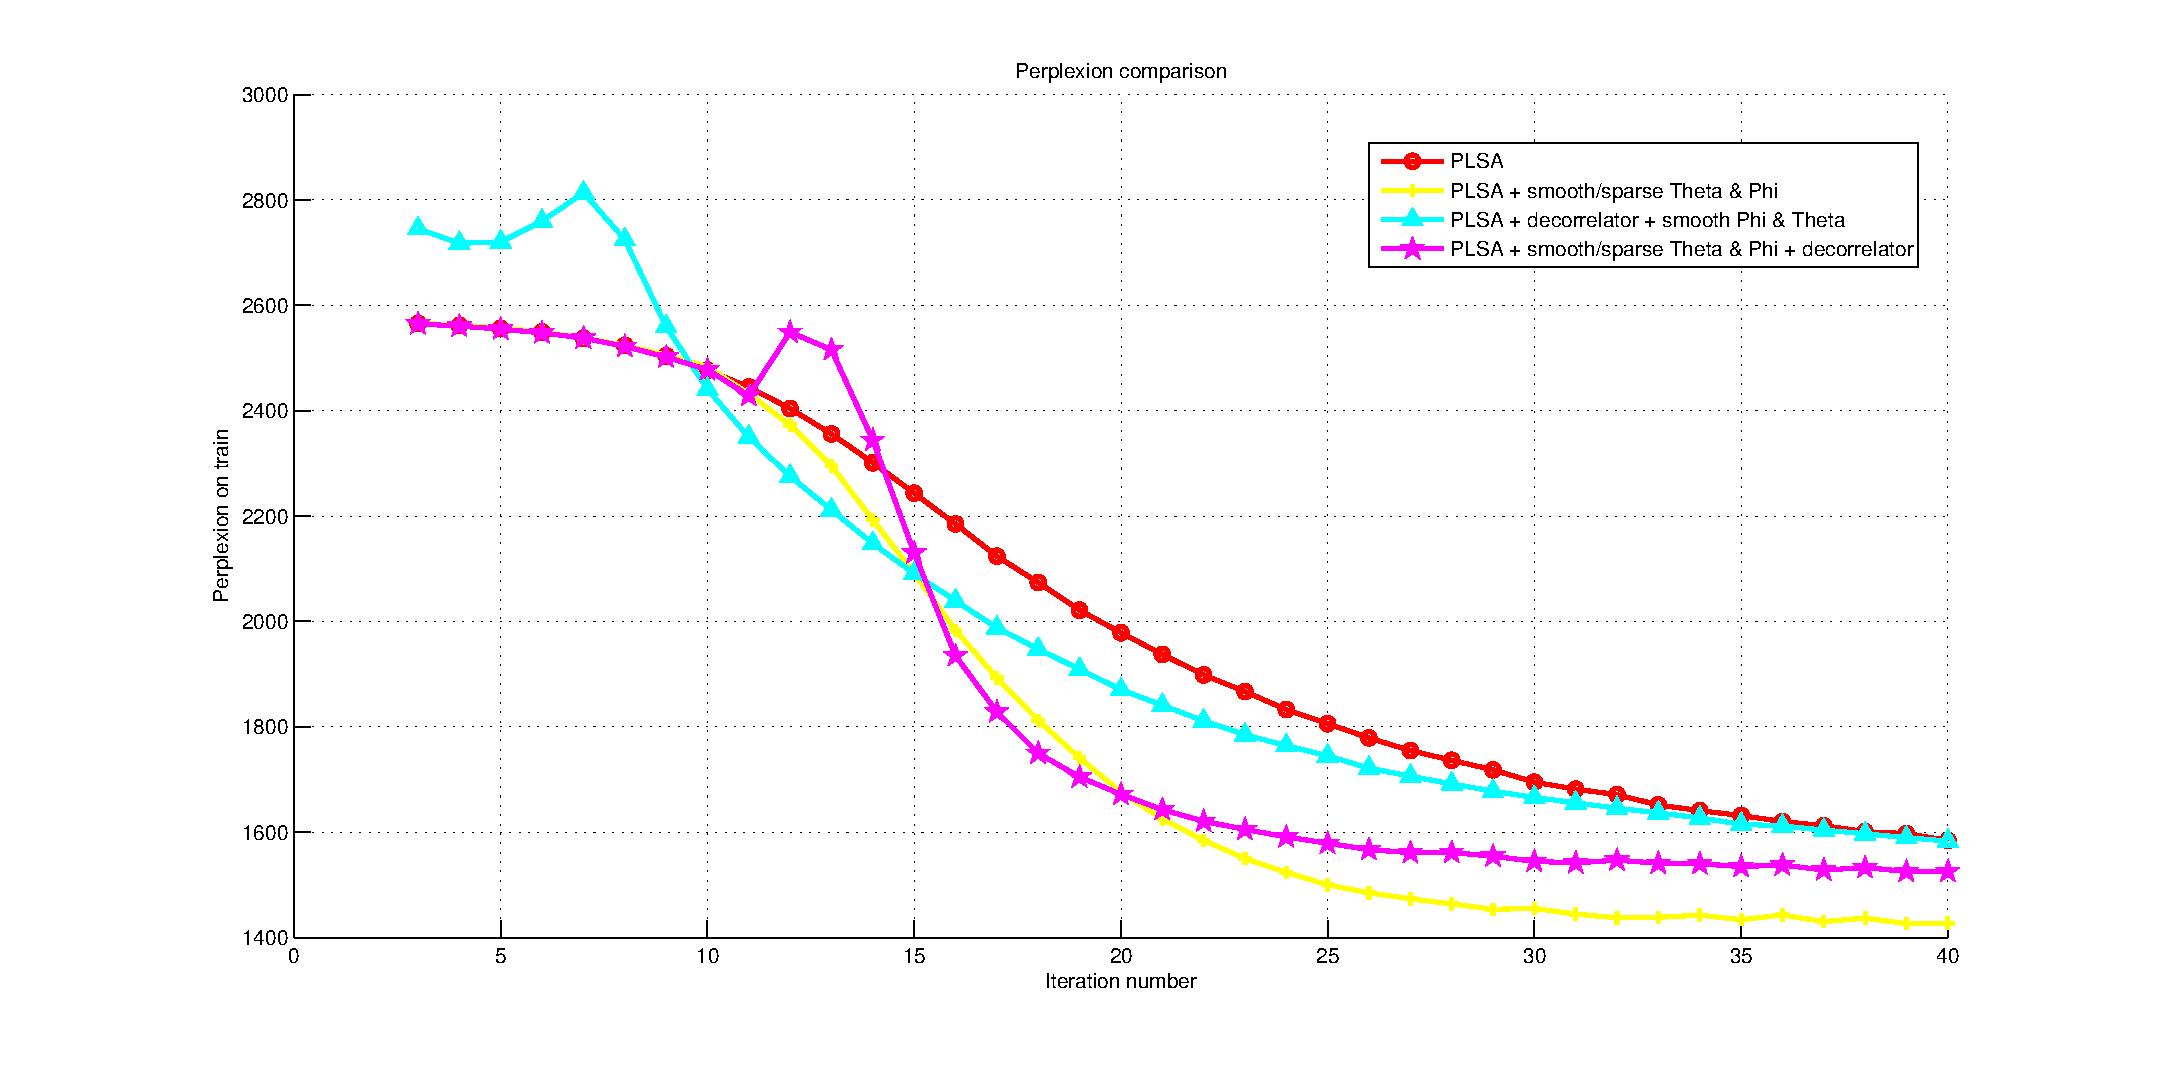
\includegraphics[scale = 0.5]{perplex.eps}
\caption{Ось X --- номер внешней итерации, ось Y --- перплексия моделей на обучающей выборке.}
\end{figure}

\begin{figure}[h!]\center
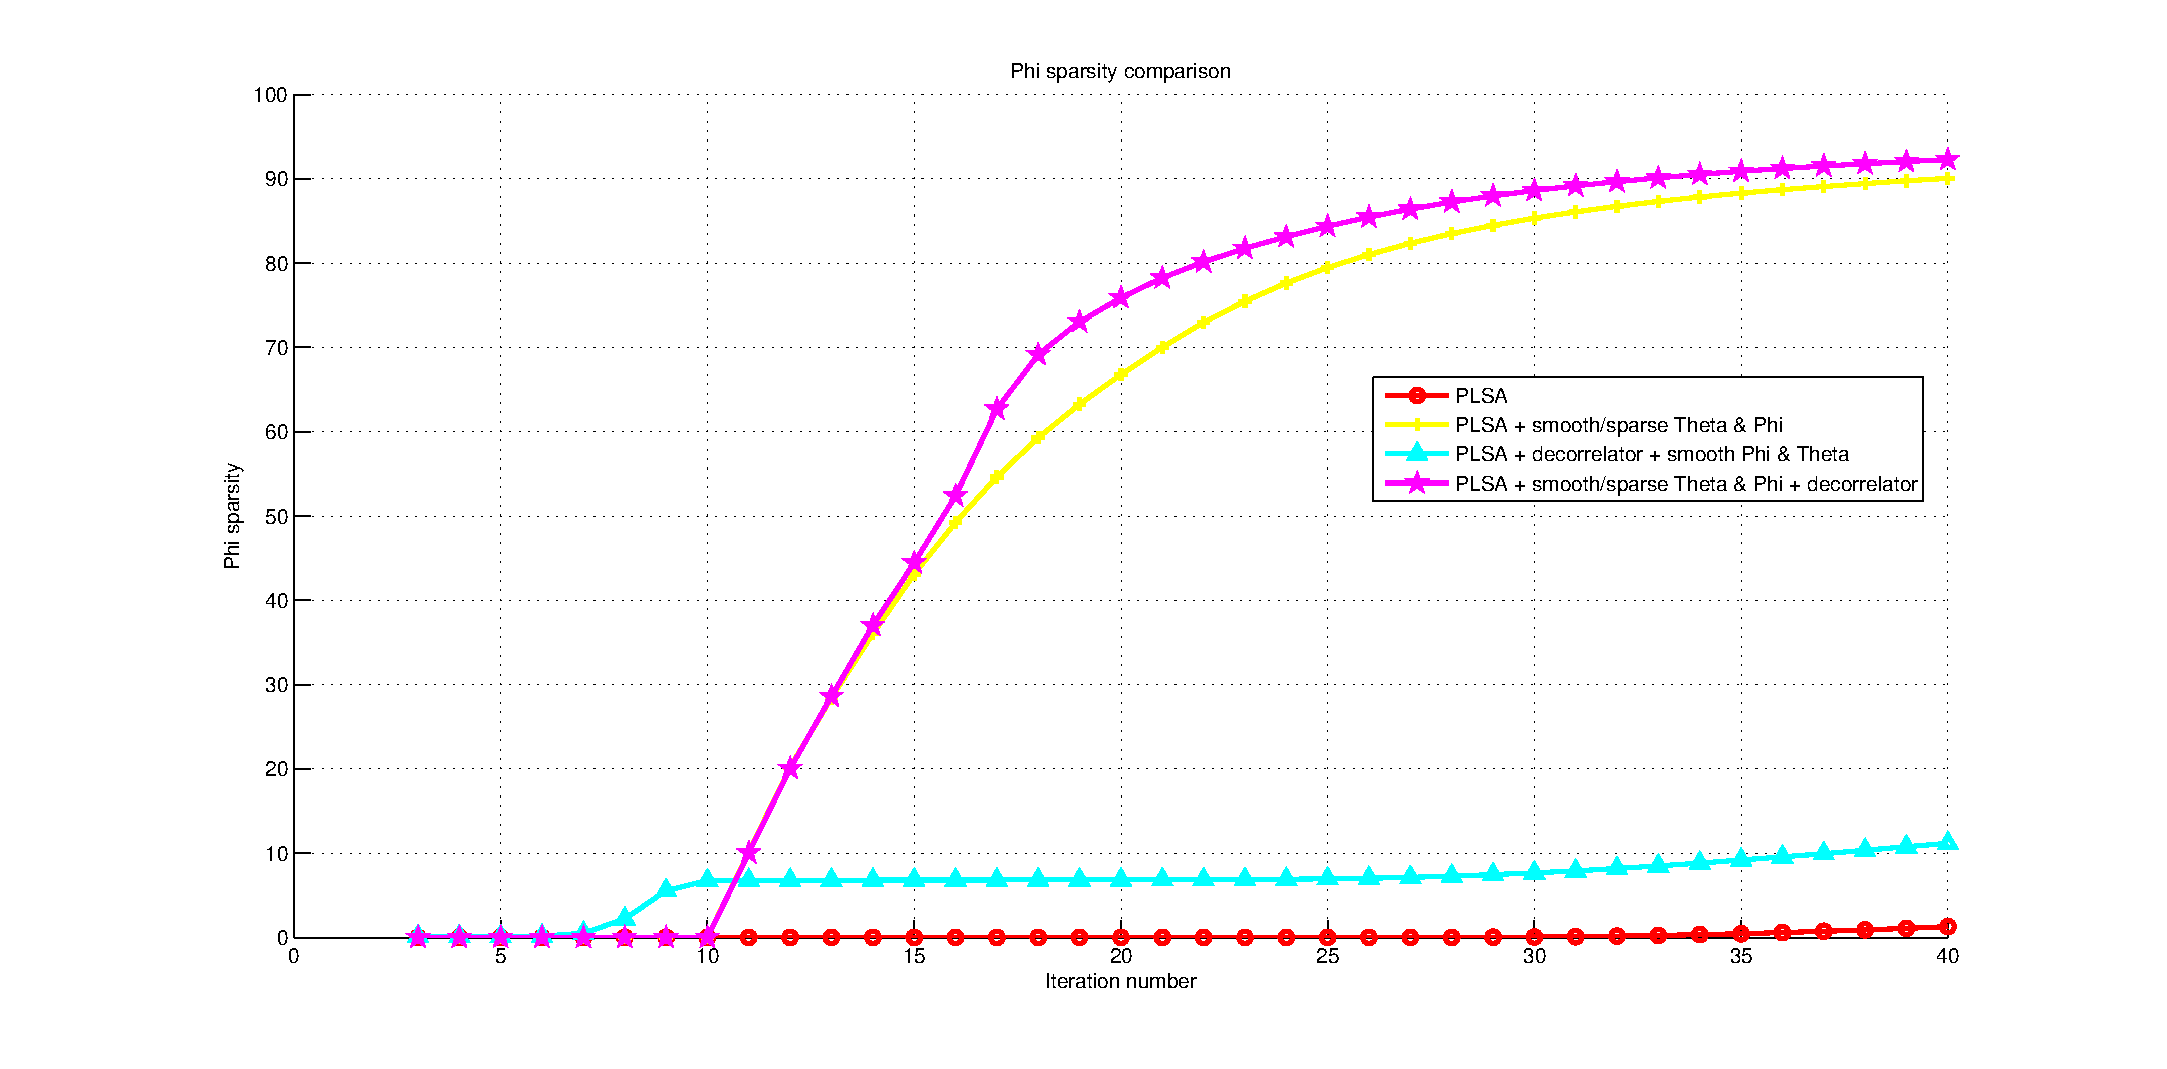
\includegraphics[scale = 0.5]{phi_sp.eps}
\caption{Ось X --- номер внешней итерации, ось Y --- разреженность матрицы $\Phi$ моделей.}
\end{figure}

\begin{figure}[h!]\center
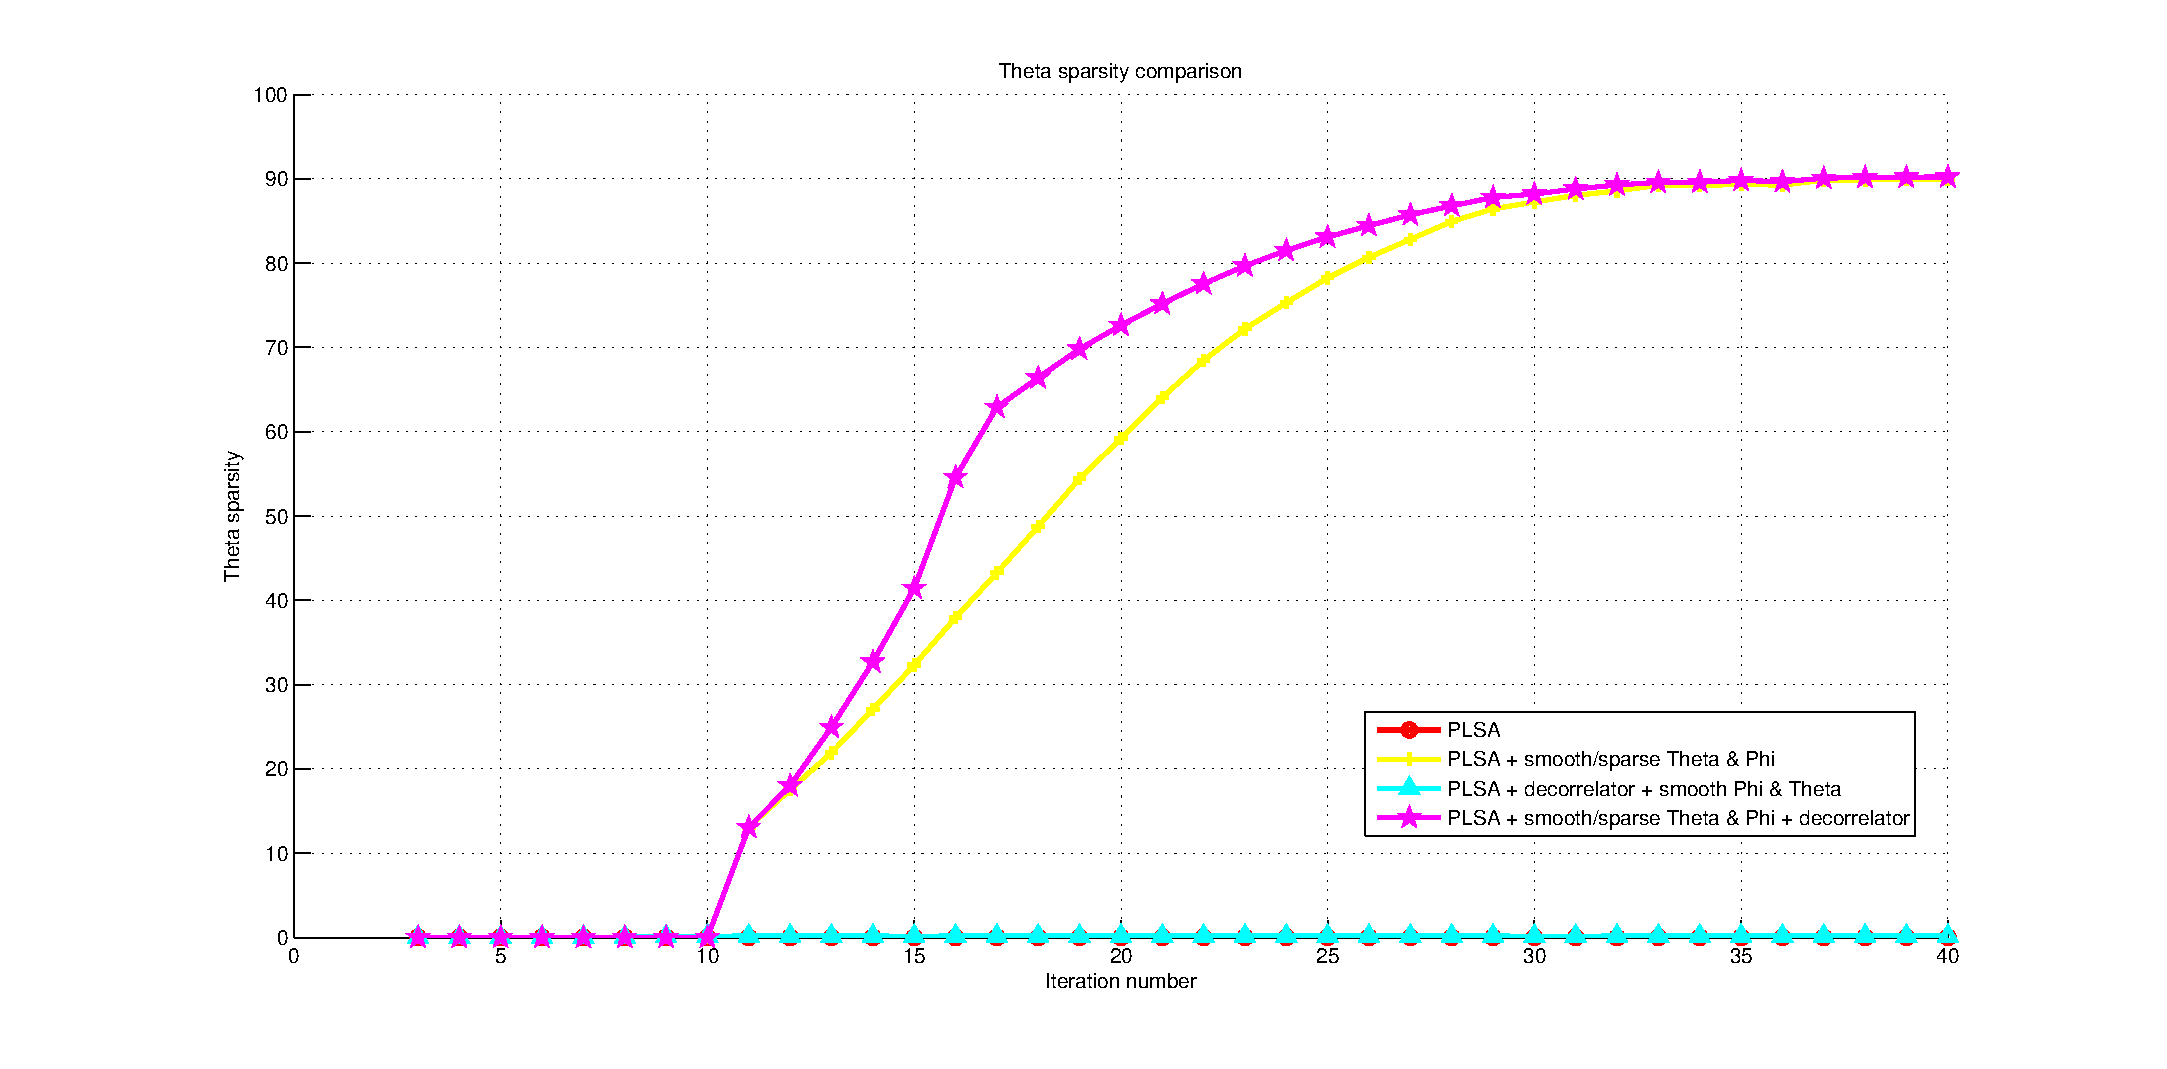
\includegraphics[scale = 0.5]{theta_sp.eps}
\caption{Ось X --- номер внешней итерации, ось Y --- разреженность матрицы $\Theta$ моделей.}
\end{figure}

\begin{figure}[h!]\center
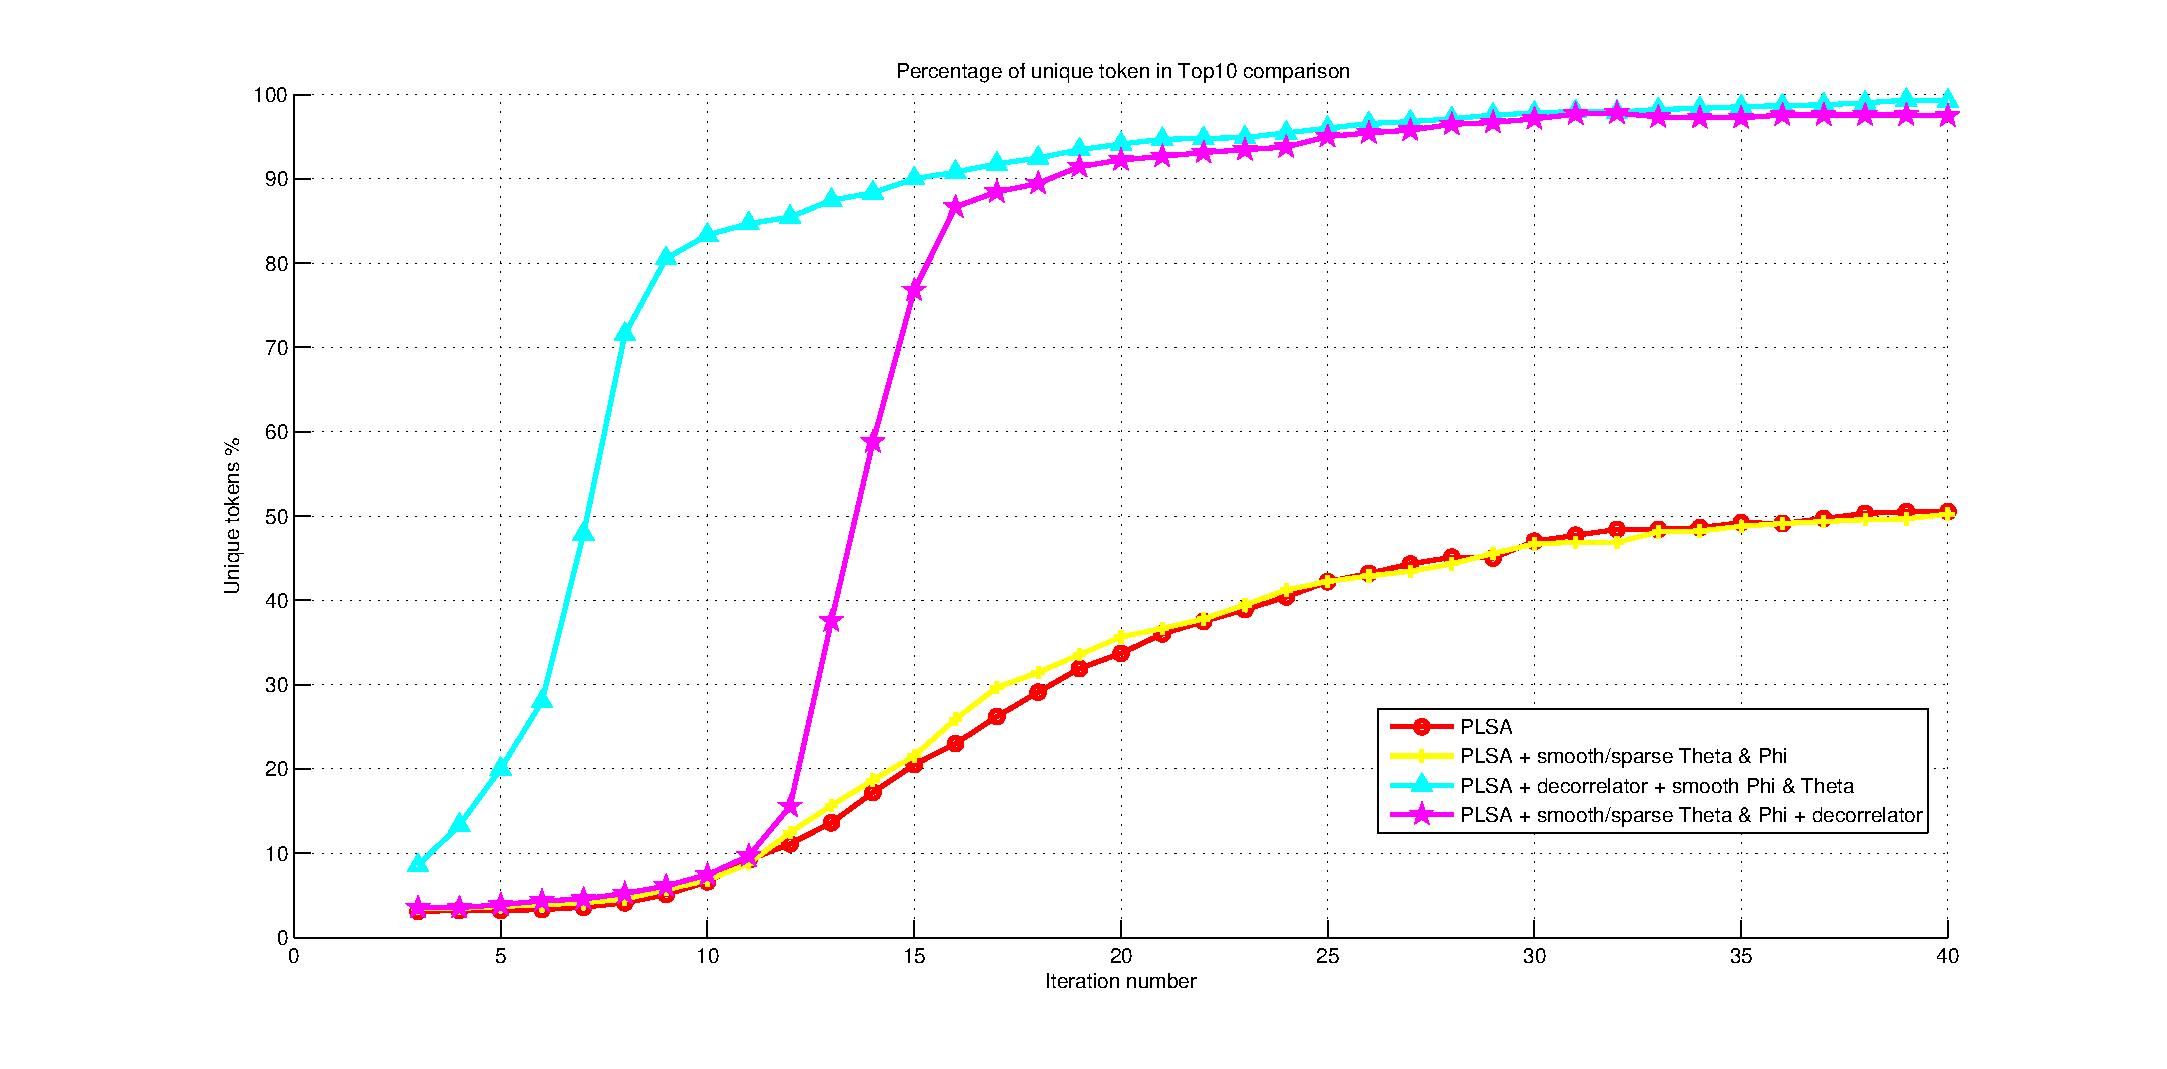
\includegraphics[scale = 0.5]{top10.eps}
\caption{Ось X --- номер внешней итерации, ось Y --- процент уникальных слов в Топ 10.}
\end{figure}

\begin{figure}[h!]\center
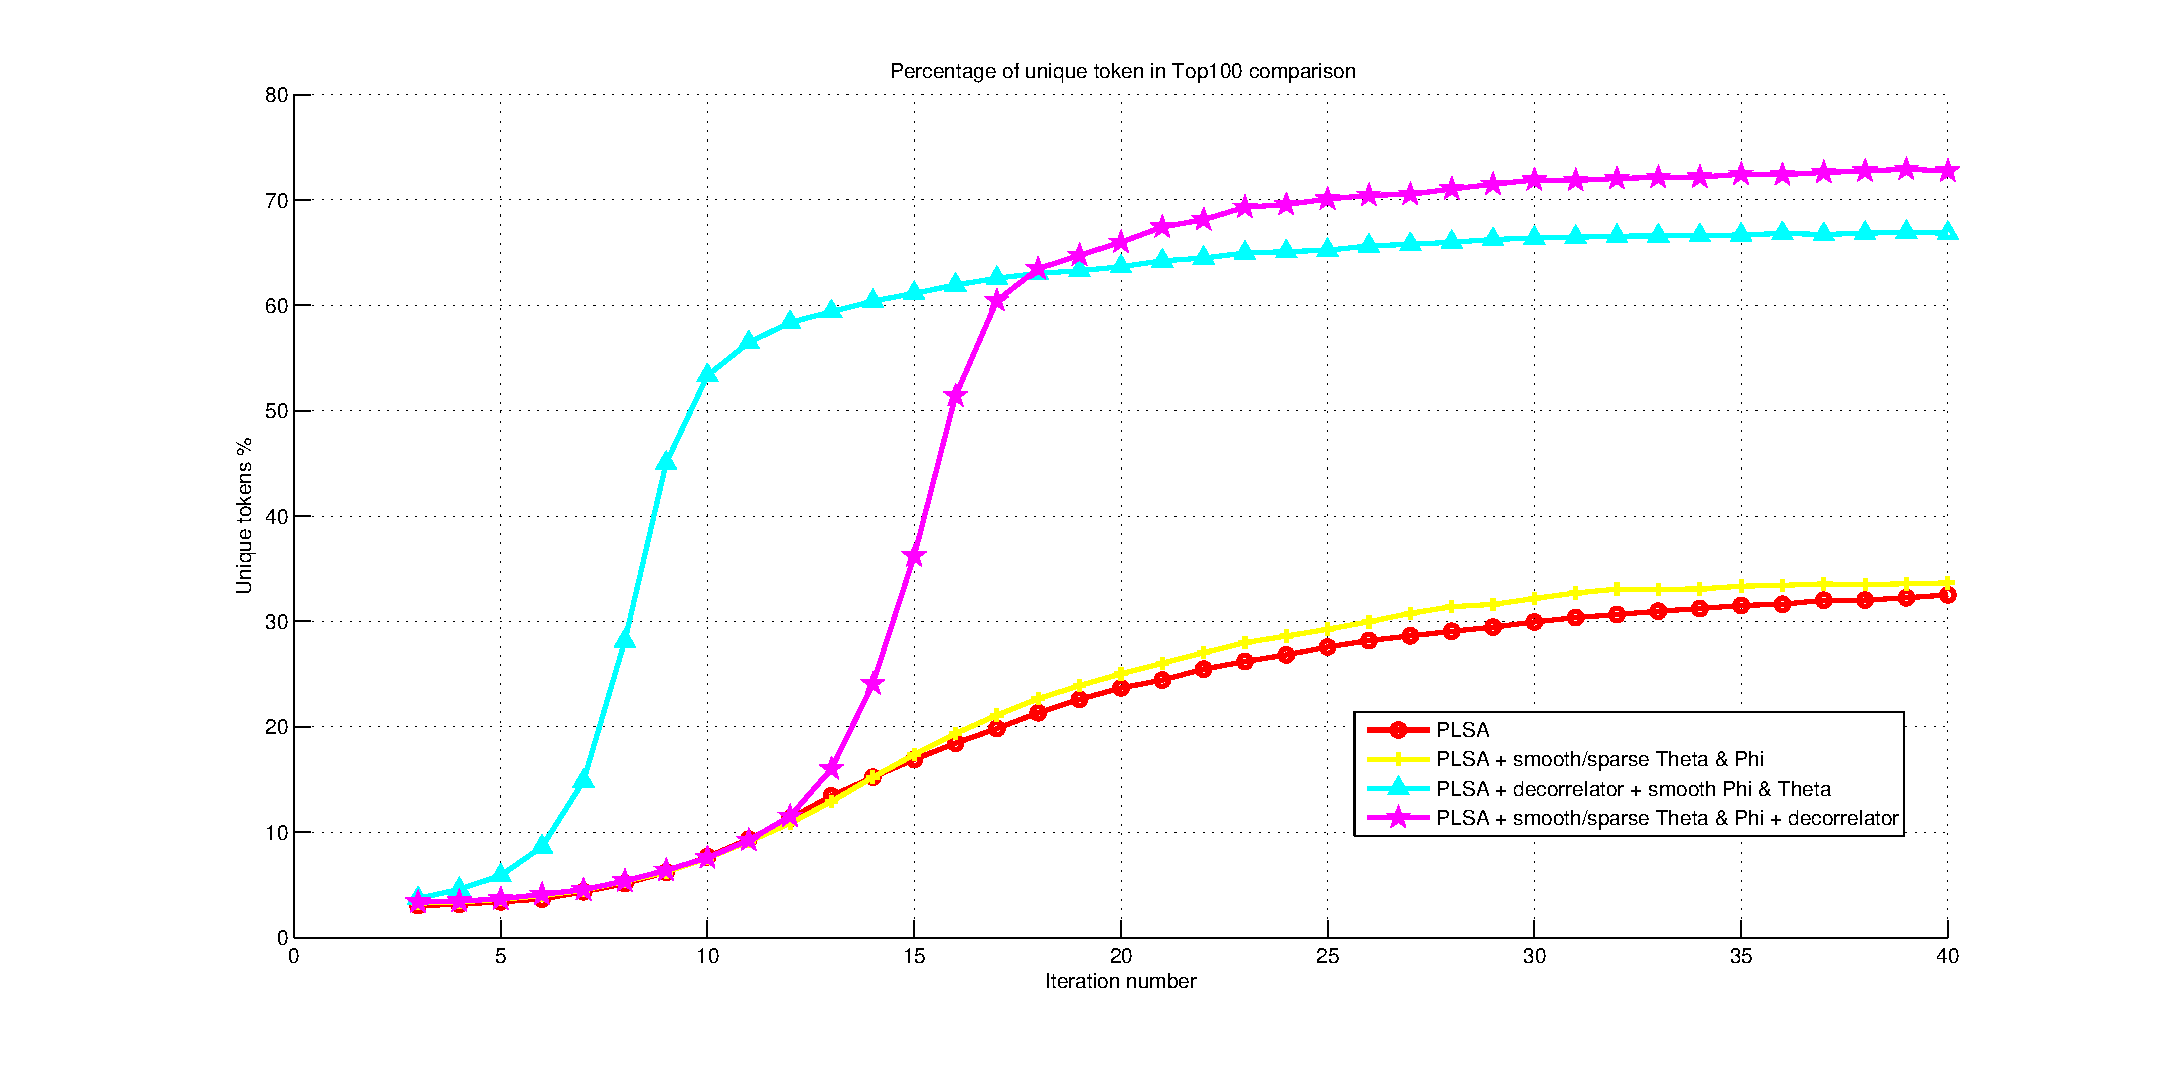
\includegraphics[scale = 0.5]{top100.eps}
\caption{Ось X --- номер внешней итерации, ось Y --- процент уникальных слов в Топ 100.}
\end{figure}